\documentclass[tikz, border=2mm]{standalone}
\usepackage{tikz}
\usetikzlibrary{calc}

\begin{document}
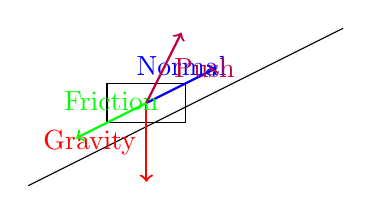
\begin{tikzpicture}
% Define the plane
\draw (0,0) -- (4,2);

% Define the block
\draw ($(1,0.8) + (0,0)$) rectangle ++(1,0.5);

% Define force vectors
\draw[->,red, thick] (1.5,1.05) -- ++(0,-1) node[midway,left] {Gravity};
\draw[->,blue, thick] (1.5,1.05) -- ++(0.8944,0.4472) node[midway,above] {Normal};
\draw[->,green, thick] (1.5,1.05) -- ++(-0.8944,-0.4472) node[midway,above] {Friction};
\draw[->,purple, thick] (1.5,1.05) -- ++(0.4472,0.8944) node[midway,right] {Push};

\end{tikzpicture}
\end{document}